\chapter{Klassenbeschreibung und Klassendiagramm}
	\newcommand{\class}[1]{\paragraph{Klasse #1:}\ \\ }
	\newcommand{\interface}[1]{\paragraph{Interface #1:}\ \\ }
	\newcommand{\method}[1]{\textcolor{blue}{#1}}
	\newcommand{\kursiv}[1]{{\it #1}}
	\newcommand{\override}{{\it @Override}\ \\}
	
	Dieses Kapitel dient der Aufführung der Klassenbeschreibung und der Darstellung des UML - Klassendiagramms der Anwendung \textbf{ofCourse}.
	Um eine bessere Übersicht und Strukturierung zu erhalten, wird das ganze Projekt in Packages aufgeteilt.\\
	Die Packagestruktur ist wie folgt aufgebaut: de.ofCourse.PACKAGENAME.\\
	\ \\
	Eine detaillierte Beschreibung der Klassen ist in dem beigefügten Dokument \kursiv{Klassenbeschreibung ofCourse} zu finden.\\
	\ \\
	Die verwendeten Synchronizations, Injections und Scopes werden im Folgenden kurz zusammenfassend
	beschrieben.\\
	\begin{itemize}
		\item \textbf{Synchronizations}\\
		Die Anwendung \textbf{ofCourse} kommt, mit einer einzigen Ausnahme ohne den Modifier \kursiv{synchronized} aus. Diese Ausnahme stellt die Klasse \kursiv{DatabaseConnectionManager} mit ihren Methoden \kursiv{getConnection()}  und \kursiv{releaseConnection()} dar.
		\item \textbf{Injections}\\
		Alle Klassen des Package \kursiv{action}, außer die Klasse \kursiv{SessionUserBean} und die Klasse
		\kursiv{MailBean}  enthalten ein \kursiv{private SessionUserBean sessionUser} Attribut, welches mit \kursiv{@ManagedProperty("\#sessionUser")} gekennzeichnet
		ist. Somit wird in diese Klassen die \kursiv{SessionUserBean} Klasse
		über Injection eingebunden.
		In der Klasse \kursiv{ContactUsersBean} wird zusätzlich zu der oben genannten Injection noch die Klasse \kursiv{MailBean}
		eingebunden.
		\item \textbf{Scopes} \\
		Alle Klassen des Package \kursiv{action} haben Scopes. Zusätzlich hat auch noch die Klasse \kursiv{LaunchSystem} aus dem Package \kursiv{system} einen Scope. Sie ist neben der Klasse \kursiv{MailBean} die einzige Klasse, welche mit \kursiv{@ApplicationScoped} annotiert ist.\\ Die Klasse \kursiv{SessionUserBean}, welche die Informationen der Session des Users speichert, ist systemweit die einzige Klasse, welche die Annotation \kursiv{@SessionScoped}  besitzt.\\ Alle Klassen, die die Funktionalität von Pagination implementieren, besitzen die Annotation \kursiv{@ViewScoped}.\\ Die restlichen Klassen, die einen Scope besitzen, sind alle mit \kursiv{@RequestScoped} annotiert.
	\end{itemize}
	
	
	\section{Klassendiagramm}
	\begin{tiny}
		Diagramm: SeSc und TF\\
	\end{tiny}\\
	Aus Gründen der Übersichtlichkeit im gesamten Klassendiagramm und da das Interface \kursiv{Transaction} und die damit verbundene Vergabe von Verbindungen zur Datenbank für unser System spezifisch ist, wird dieses exemplarisch in einem separaten Beispielfall in einem Klassendiagramm \ref{fig:Teildiagramm} dargestellt.
	\begin{figure}[h]
	\centering
	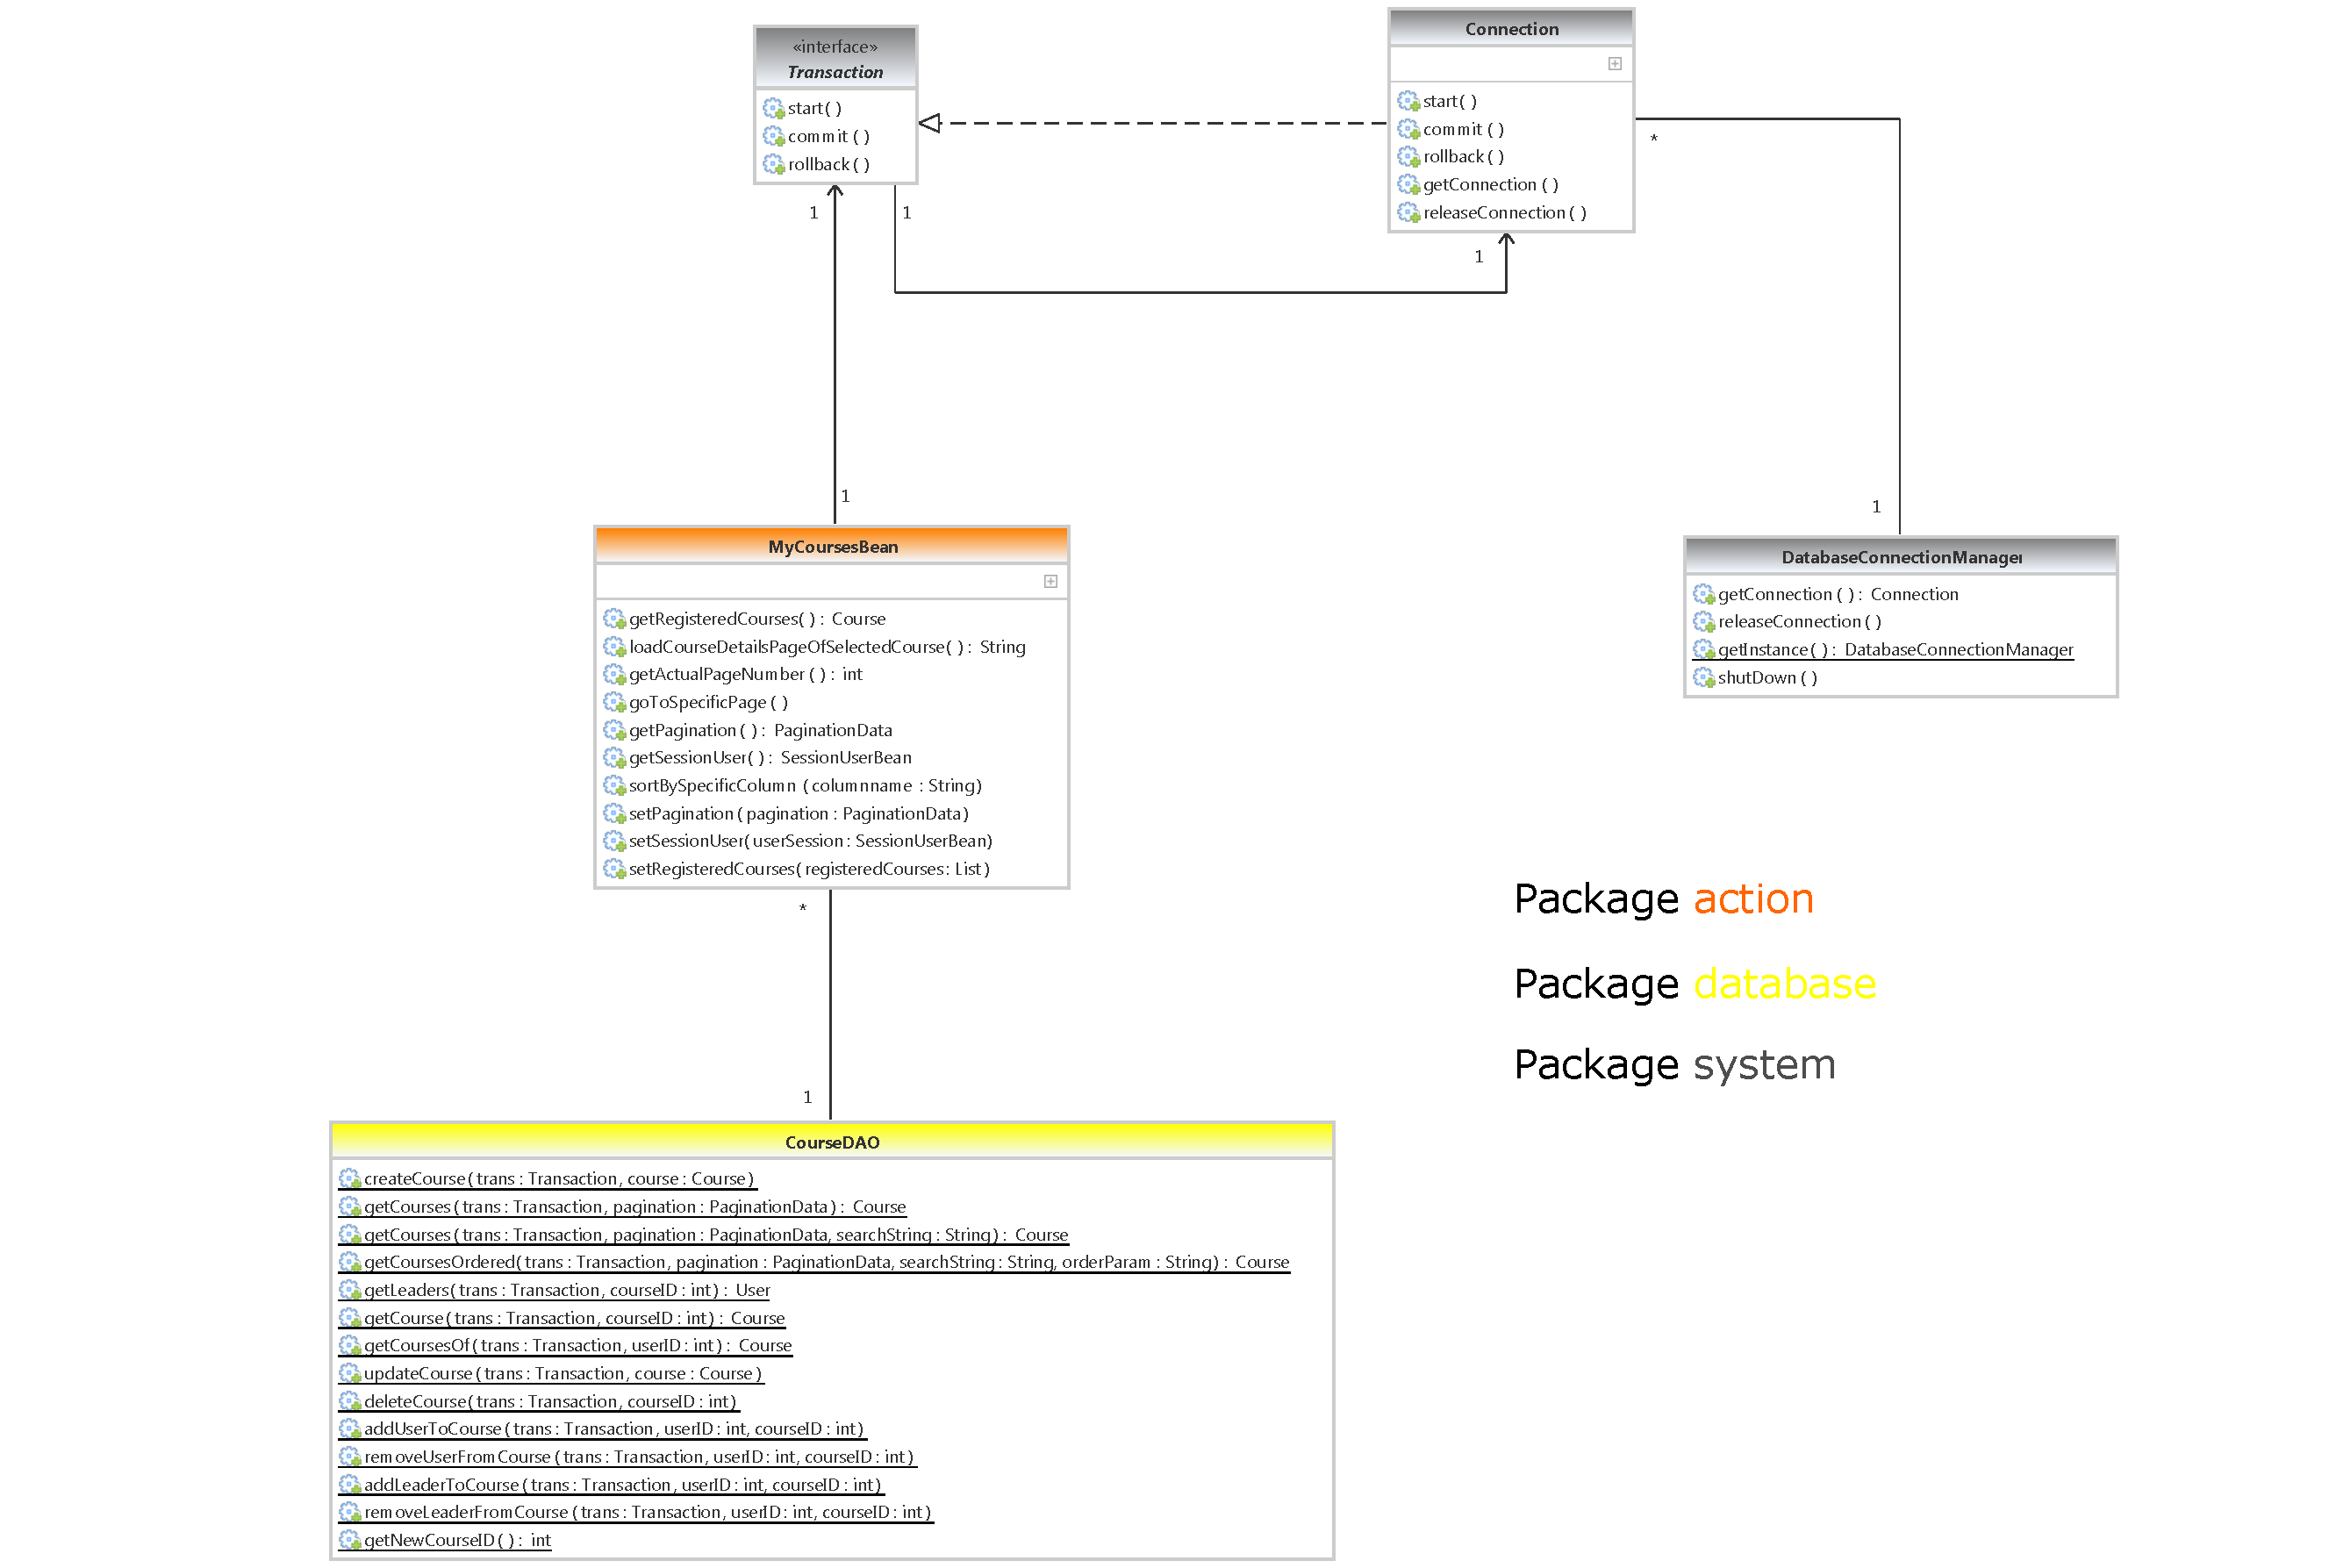
\includegraphics[width=1\linewidth]{Grafiken/Teildiagramm}
	\caption{UML-Teildiagramm zum Interface Transaction}
	\label{fig:Teildiagramm}
	\end{figure}
	\ \\
	In der nachfolgenden Abbildung \ref{fig:UMLKlassendiagrammOhneTransaction_ink} ist das UML-Klassendiagramm des \textbf{ofCourse-Systems} dargestellt.\\
	Um sich dieses Diagramm genauer ansehen zu können, muss es mit einem PDF-Reader
	geöffnet werden, der eine Zoom-Funktion besitzt.
	
	\begin{figure}[h]
	\centering
	\includegraphics[width=1\linewidth, angle=90]{Grafiken/UMLKlassendiagrammOhneTransaction_ink}
	\caption{UML-Klassendiagramm des ofCourse-Systems}
	\label{fig:UMLKlassendiagrammOhneTransaction_ink}
	\end{figure}
	
